\section{Business Process Modelling}

\begin{exercise}{1}
Using only the base BPMN elements (activities, gateways and sequence flows), model the following process:
\\\\An order-to-cash process is triggered by the receipt of a purchase order from a customer. 
Upon receipt, the purchase order has to be checked against the stock to determine if the requested item(s) are available.
Depending on stock availability thepurchase order may be confirmed or rejected.
If the purchase order is rejected, the process completes.
If the purchase order is confirmed, an invoice is emitted, and the goods requested are shipped.
\end{exercise}
\paragraph{Solution:}
\begin{figure}[H]
    \centering
    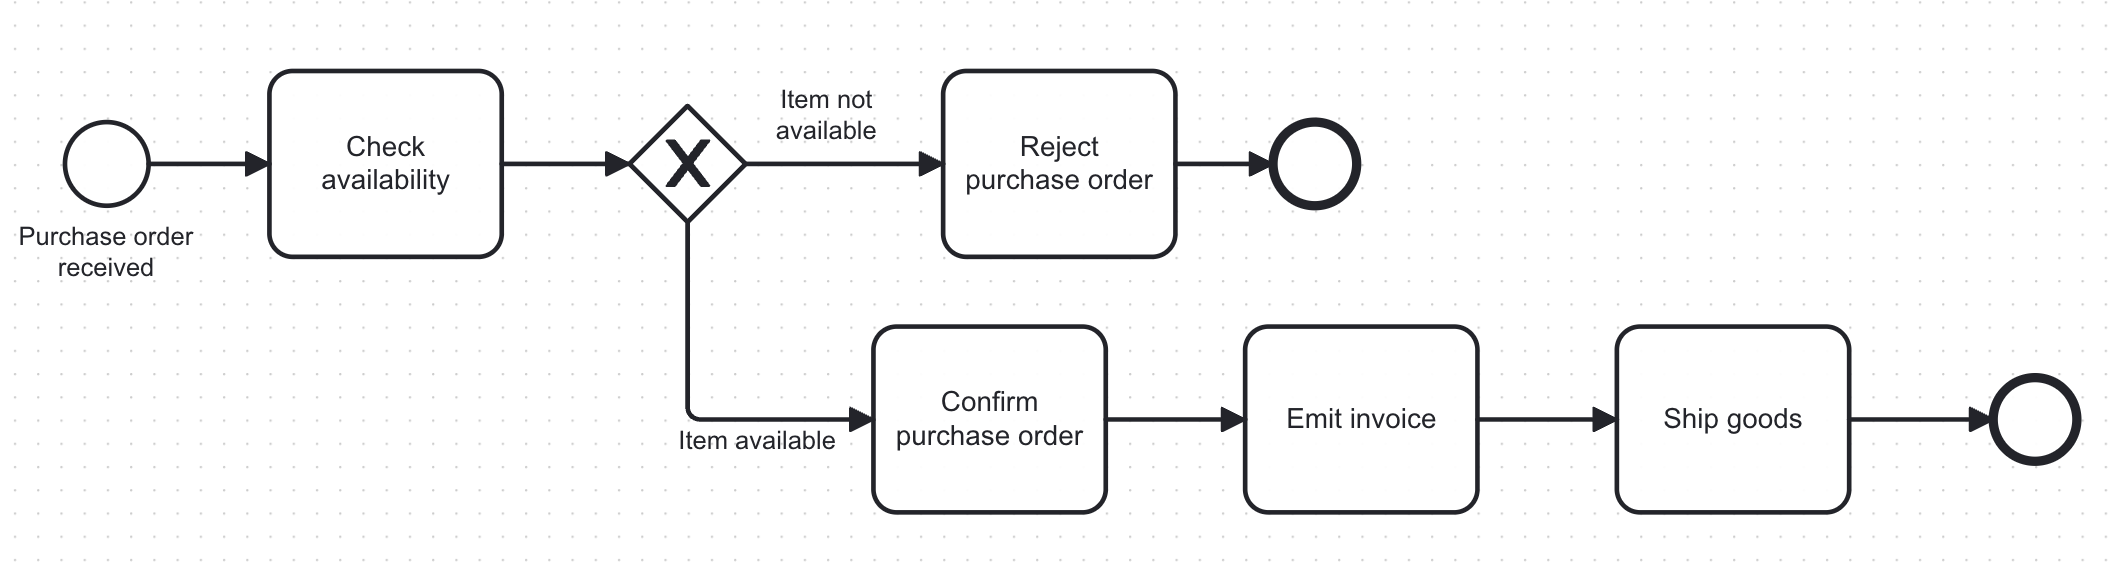
\includegraphics[width=\textwidth]{../images/exercises/bpmn/bpmn-1.png}
    \caption{Solution for Exercise 1}
\end{figure}
The solution here is pretty straightforward:
\begin{itemize}
    \item A process instance starts with the receipt of a purchase order from a customer (start event);
    \item The purchase order is checked against the stock (activity);
    \item A gateway checks if the items are available in stock:
    \begin{itemize}
        \item If the items are not available, the purchase order is rejected (activity) and the process ends (end event);
        \item If the items are available, the purchase order is confirmed (activity), an invoice is emitted (activity), and the goods requested are shipped (activity), then the process ends (end event).
    \end{itemize}
\end{itemize}

\begin{exercise}{2}
Using only the base BPMN elements (activities, gateways and sequence flows), model the following process:
\\\\Once a loan application has been approved, an
acceptance pack is prepared and sent to the customer.
The acceptance pack includes a repayment schedule,
which the customer needs to agree upon. The payment
documents are received back by the loan provider. The
latter then verifies the repayment agreement: if the
applicant disagreed with the repayment schedule, the
loan provider cancels the application; if the applicant
agreed, the loan provider approves the application. In
either case, the loan completes with the loan provider
notifying the applicant of the application status.
\end{exercise}
\paragraph{Solution:}
\begin{figure}[H]
    \centering
    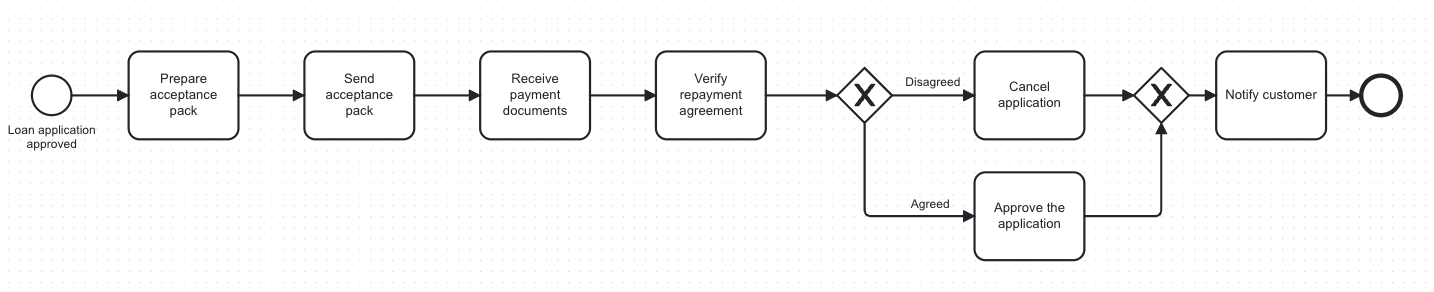
\includegraphics[width=\textwidth]{../images/exercises/bpmn/bpmn-2.png}
    \caption{Solution for Exercise 2}
\end{figure}
The solution here is as follows:
\begin{itemize}
    \item A process instance starts with the approval of a loan application (start event);
    \item An acceptance pack is prepared and sent to the customer (activity);
    \item The payment documents are received back by the loan provider (activity) and the repayment agreement is verified (activity);
    \item A XOR split gateway checks if the applicant agreed with the repayment schedule:
    \begin{itemize}
        \item If the applicant disagreed, the loan application is cancelled (activity);
        \item If the applicant agreed, the loan application is approved (activity).
    \end{itemize}
    \item In either case (XOR JOIN) the loan completes with the notification of the applicant of the application status (activity).
\end{itemize}

\begin{exercise}{3}
Using only the base BPMN elements (activities, gateways and sequence flows), model the following process:
\\\\In the minister’s office, when a ministerial inquiry has been received, it
is assigned to be registered into the system. Then the inquiry is
investigated so that a ministerial response can be prepared.
\\The finalization of a response includes the preparation of the response
itself by the cabinet officer and the review of the response by the
principal registrar. If the registrar does not approve the response, the
latter needs to be prepared again by the cabinet officer for review. The
process finishes only once the response has been approved.
\end{exercise}
\paragraph{Solution:}
\begin{figure}[H]
    \centering
    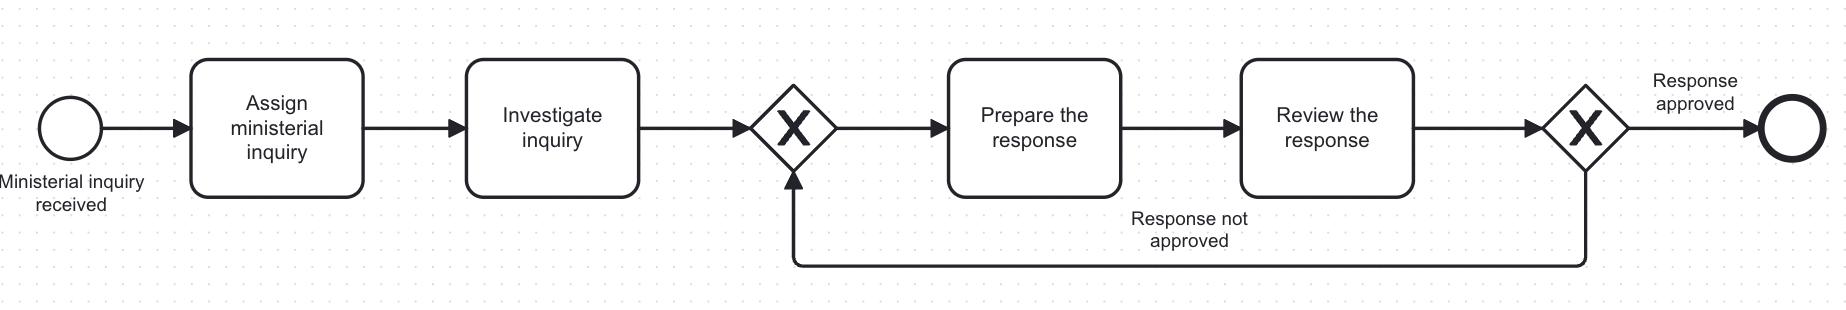
\includegraphics[width=\textwidth]{../images/exercises/bpmn/bpmn-3.png}
    \caption{Solution for Exercise 3}
\end{figure}
The solution here is as follows:
\begin{itemize}
    \item A process instance starts with the receipt of a ministerial inquiry (start event);
    \item The inquiry is assigned to be registered (activity) and then investigated (activity);
    \item Since if the response is not approved it needs to be prepared again, we have a rework loop here:
    \begin{itemize}
        \item A XOR JOIN gateway signals the entry point of the loop;
        \item The response is prepared by the cabinet officer (activity);
        \item The response is reviewed by the principal registrar (activity);
        \item A XOR split gateway checks if the registrar approves the response:
        \begin{itemize}
            \item If it is approved, the process ends (end event);
            \item If it is not approved, the flow goes back to the XOR JOIN gateway to re-enter the loop.
        \end{itemize}
    \end{itemize}
\end{itemize}

\begin{exercise}{4}
Using only the base BPMN elements (activities, gateways and sequence flows), model the following process:
\\\\Once received, a loan application is approved if it passes two checks: 
\begin{enumerate}
    \item the applicant’s loan risk assessment;
    \item the appraisal of the property for which the loan has been asked.
\end{enumerate}
The risk assessment requires a credit history check on the applicant.
Once both the loan risk assessment and the process appraisal have been performed, the applicant’s eligibility can be assessed.
If the applicant is not eligible, the application is rejected,
otherwise the acceptance pack is prepared and sent to the applicant.
\end{exercise}
\paragraph{Solution:}
\begin{figure}[H]
    \centering
    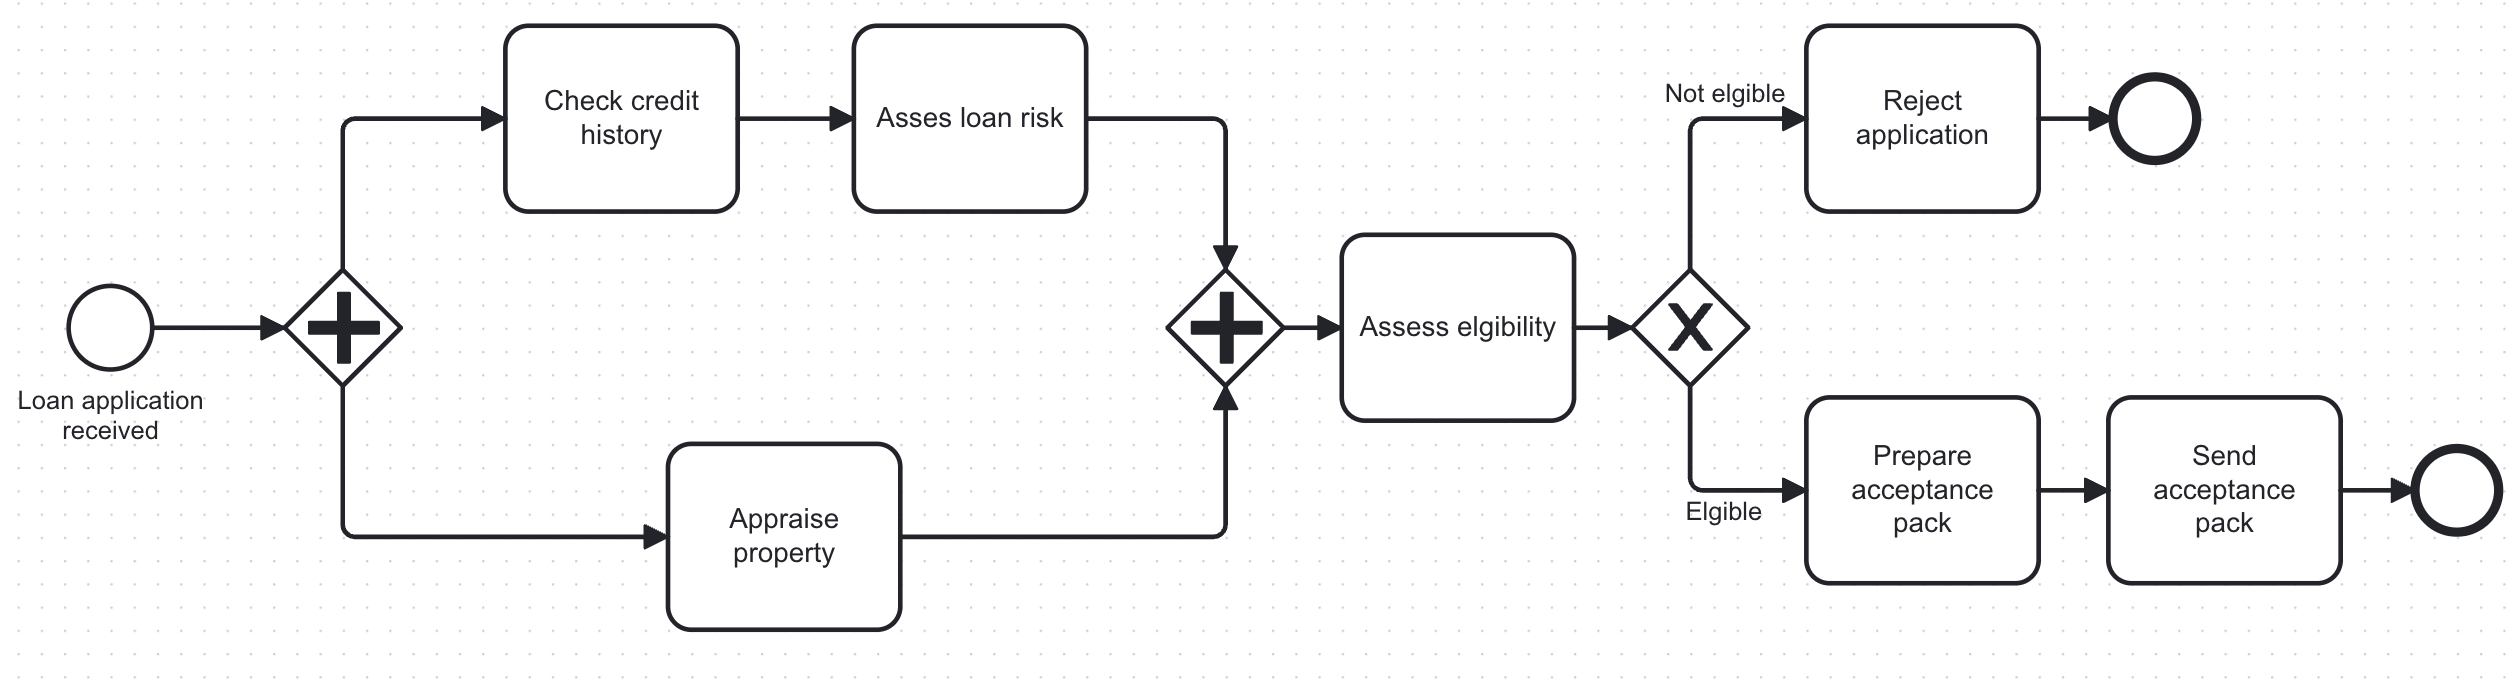
\includegraphics[width=\textwidth]{../images/exercises/bpmn/bpmn-4.png}
    \caption{Solution for Exercise 4}
\end{figure}
The solution here is as follows:
\begin{itemize}
    \item A process instance starts with the receipt of a loan application (start event);
\end{itemize}
\begin{itemize}
    \item A process instance starts with the receipt of a loan application (start event);
    \item because not specified otherwise, we assume that the two checks can be performed in parallel (AND split gateway):
    \begin{itemize}
        \item One branch performs the credit history check (activity) and then the loan risk assessment (activity);
        \item The other branch performs the appraisal of the property (activity). 
        \end{itemize}
    \item An AND JOIN gateway synchronizes the two branches once both checks are completed;
    \item The applicant’s eligibility is assessed (activity);
    \item A XOR split gateway checks if the applicant is eligible:
    \begin{itemize}
        \item If the applicant is not eligible, the application is rejected (activity) and the process ends (end event);
        \item If the applicant is eligible, the acceptance pack is prepared and sent to the applicant (activity) and the process ends (end event).
    \end{itemize}
\end{itemize}

\begin{exercise}{5}
Using only the base BPMN elements (activities, gateways and sequence flows) and pools/lanes, model the following process:
\\\\The order-to-cash process is carried out by a \textbf{Seller’s organization}
which includes two departments: the \textbf{Sales department} and the \textbf{Warehouse \& Distribution department}.
The purchase order received by the Seller has to be checked against
the stock. This is done automatically by an \textbf{ERP system}, which is
part of the \textbf{Warehouse \& Distribution department} together with the
\textbf{Warehouse Staff}. If the product is in stock, the \textbf{Sales department}
confirms the order. If it is not in the stock, the \textbf{Sales department}
rejects the order.
If the purchase order is confirmed, the \textbf{Warehouse Staff} in the
\textbf{Warehouse \& Distribution department} ships the goods. Meantime,
the \textbf{Sales department} emits the invoice. The process concludes with
the order being archived by the \textbf{Sales department}.
\end{exercise}
\paragraph{Solution:}
\begin{figure}[H]
    \centering
    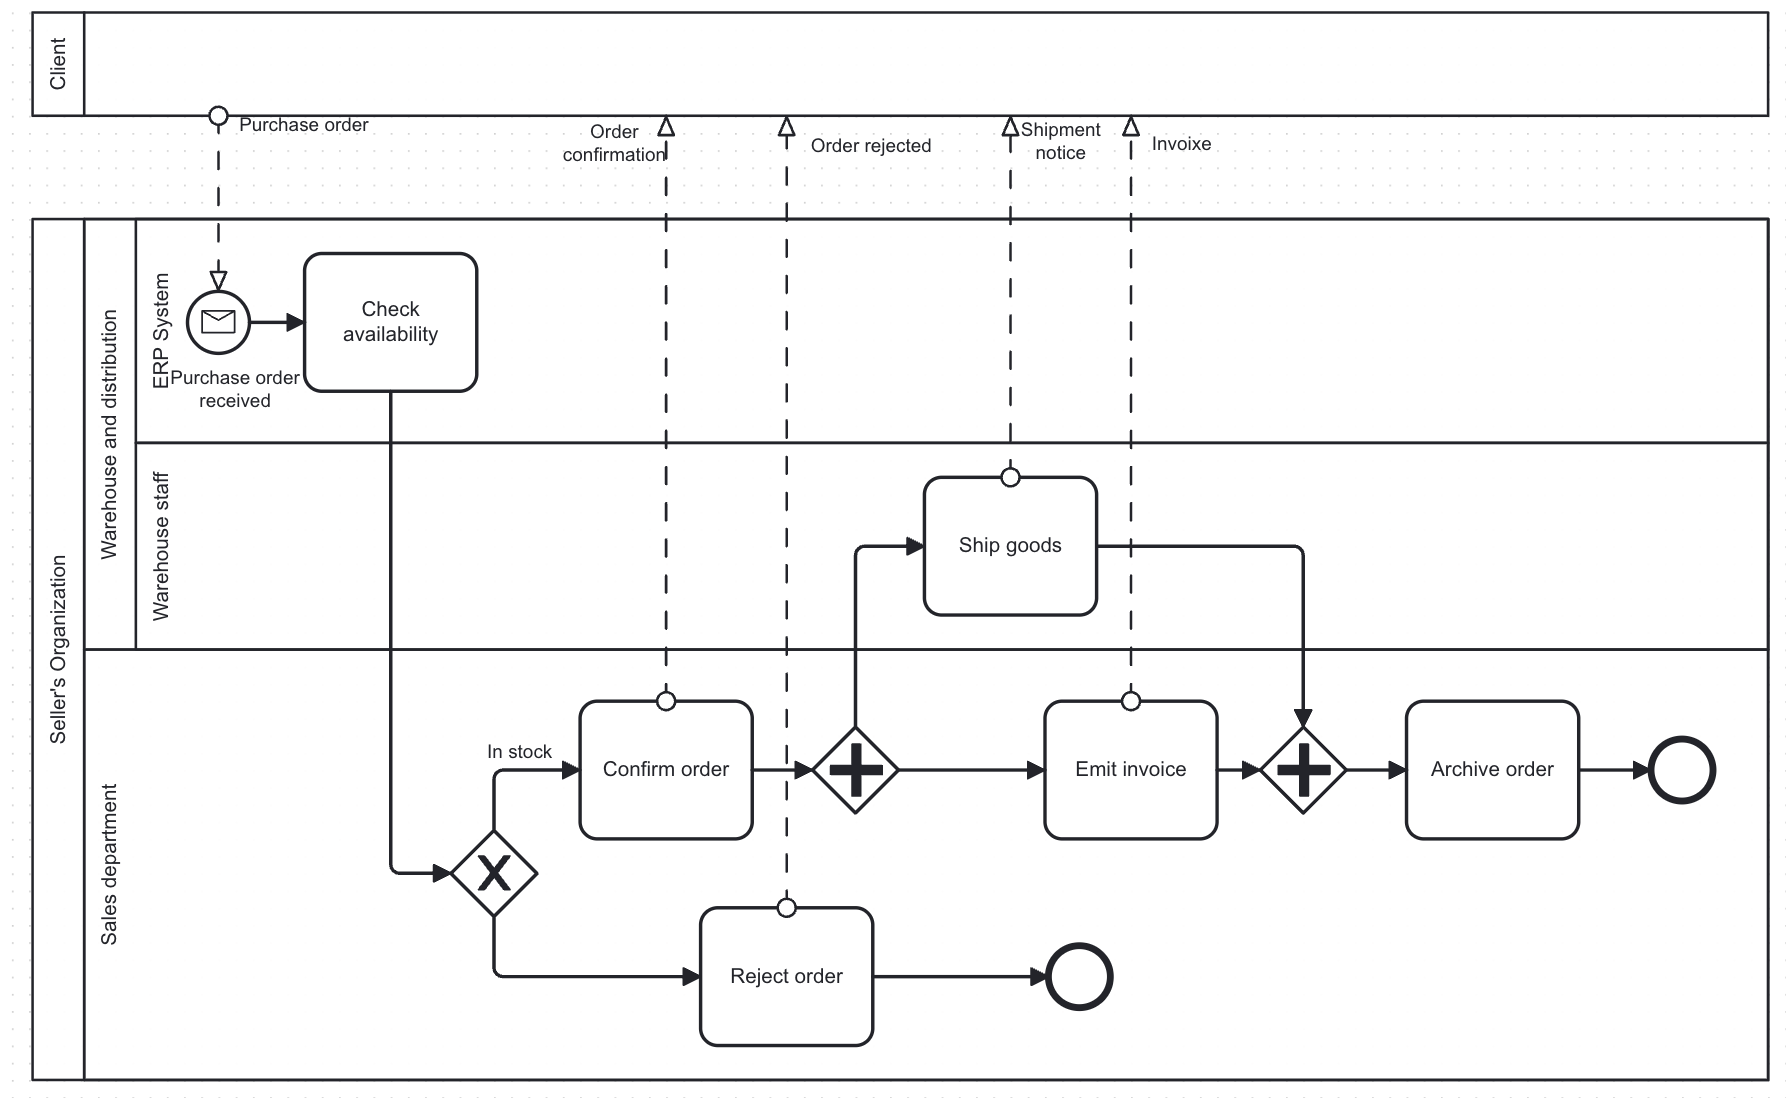
\includegraphics[width=\textwidth]{../images/exercises/bpmn/bpmn-5.png}
    \caption{Solution for Exercise 5}
\end{figure}
The solution here is as follows:
\begin{itemize}
    \item For this kind of exercise, it's adviced to first identify the basic process flow. Only then,
    identify the different participants (pools/lanes) and assign the activities to them.
    \item In this case, we have two main pools:
    \begin{itemize}
        \item The \textbf{Seller's organization} pool, which contains two lanes:
        \begin{itemize}
            \item The \textbf{Sales department} lane;
            \item The \textbf{Warehouse \& Distribution department} lane, which contains the \textbf{Warehouse Staff} and \textbf{ERP system} sub-lanes.
        \end{itemize}
        \item The \textbf{Client} pool, which represents the customer making the purchase order. 
    \end{itemize}
    \item We can then add all the message flows between the two pools (dashed lines with empty arrowheads).
\end{itemize}

\begin{exercise}{6}
Given the following process description, create a BPMN model that captures all the details:
\\\\In the context of a claim handling process, it is sometimes necessary to 
send a questionnaire to the claimant to gather additional information.
The claimant is expected to return the questionnaire within five days. 
If no response is received after five days, a reminder is sent to the claimant. 
If after another five days there is still no response, another reminder is sent 
and so on until the completed questionnaire is received.
Once the questionnaire is received, it is assessed.
\end{exercise}
\paragraph{Solution:}
\begin{figure}[H]
    \centering
    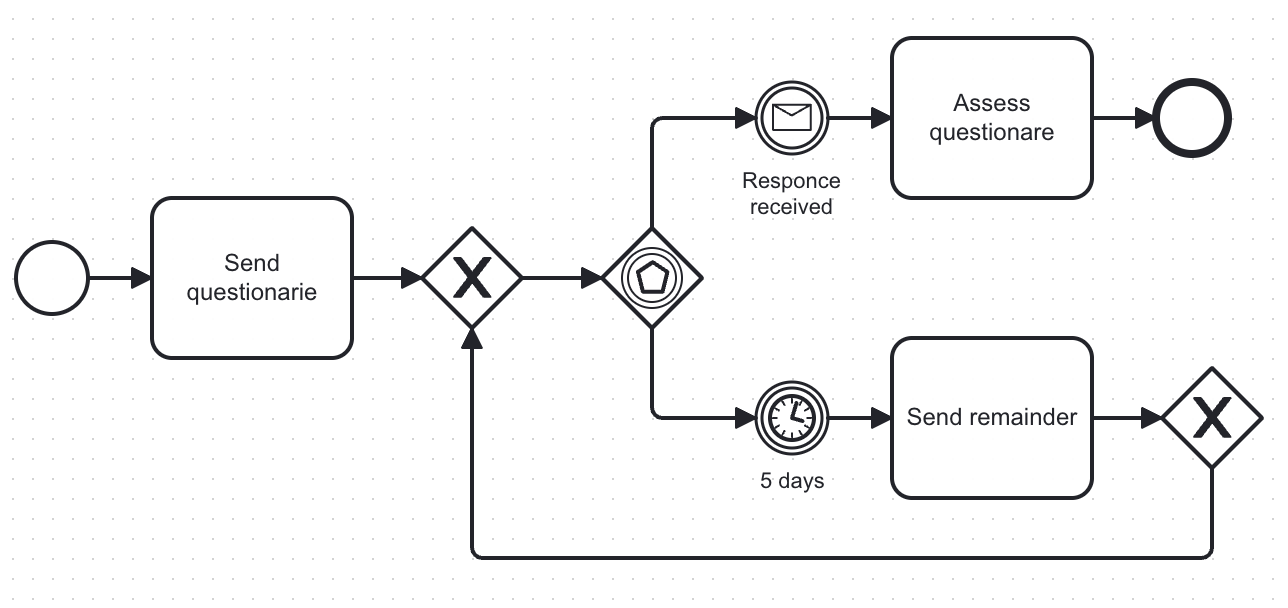
\includegraphics[width=\textwidth]{../images/exercises/bpmn/bpmn-6.png}
    \caption{Solution for Exercise 6}
\end{figure}
The notable aspect of this solution are:
\begin{itemize}
    \item The use of a block structued loop to allow any number of reminders to be sent until the questionnaire is received;
    \item The use of an event-based gateway to model the waiting for either receive the questionnaire or the timeout of five days.
    In particular:
    \begin{itemize}
        \item The intermediate timer event models the timeout of five days;
        \item The intermediate message receive event models the reception of the completed questionnaire;
    \end{itemize}
\end{itemize}

\begin{exercise}{7}
Given the following process description, create a BPMN model that captures all the details:
\\\\The clients of the IT helpdesk are employees of a company. A request may be an IT-
related problem that a client has, or an access request (e.g., requesting rights to access
an IT system). Requests need to be handled according to their type and their priority.
A client makes a request to the help desk. The help desk staffed with “Level-1” support
staff registers the request. Level-1 support staff typically are junior people with less than
12 months experience, but are capable of resolving simple requests. When the Level-1
employee knows how to resolve a request, she resolves it, notifies the resolution to the
client and closes the simple request.
When the Level-1 employee does not know how to resolve a request, the request is for-
warded to a more experienced “Level-2” support staff. When a Level-2 employee receives
a request, the request is evaluated, a resolution is developed and sent back to the Level-1
employee. Eventually, the Level-1 employee forwards the resolution to the client who
can test the resolution and notify the outcome to the IT helpdesk. The client notifies
the outcome of the test to the Level-1 employee via e-mail. If the client states that the
request is fixed, the request is closed successfully, and the process ends. If the request is
not fixed, it is resent to Level-2 support for further action and goes through the process
again. If, instead, after the client notification, no test outcome is received back for a
month, the Level-1 employee closes the request for timeout and the process ends.
\end{exercise}
\paragraph{Solution:}
\begin{figure}[H]
    \centering
    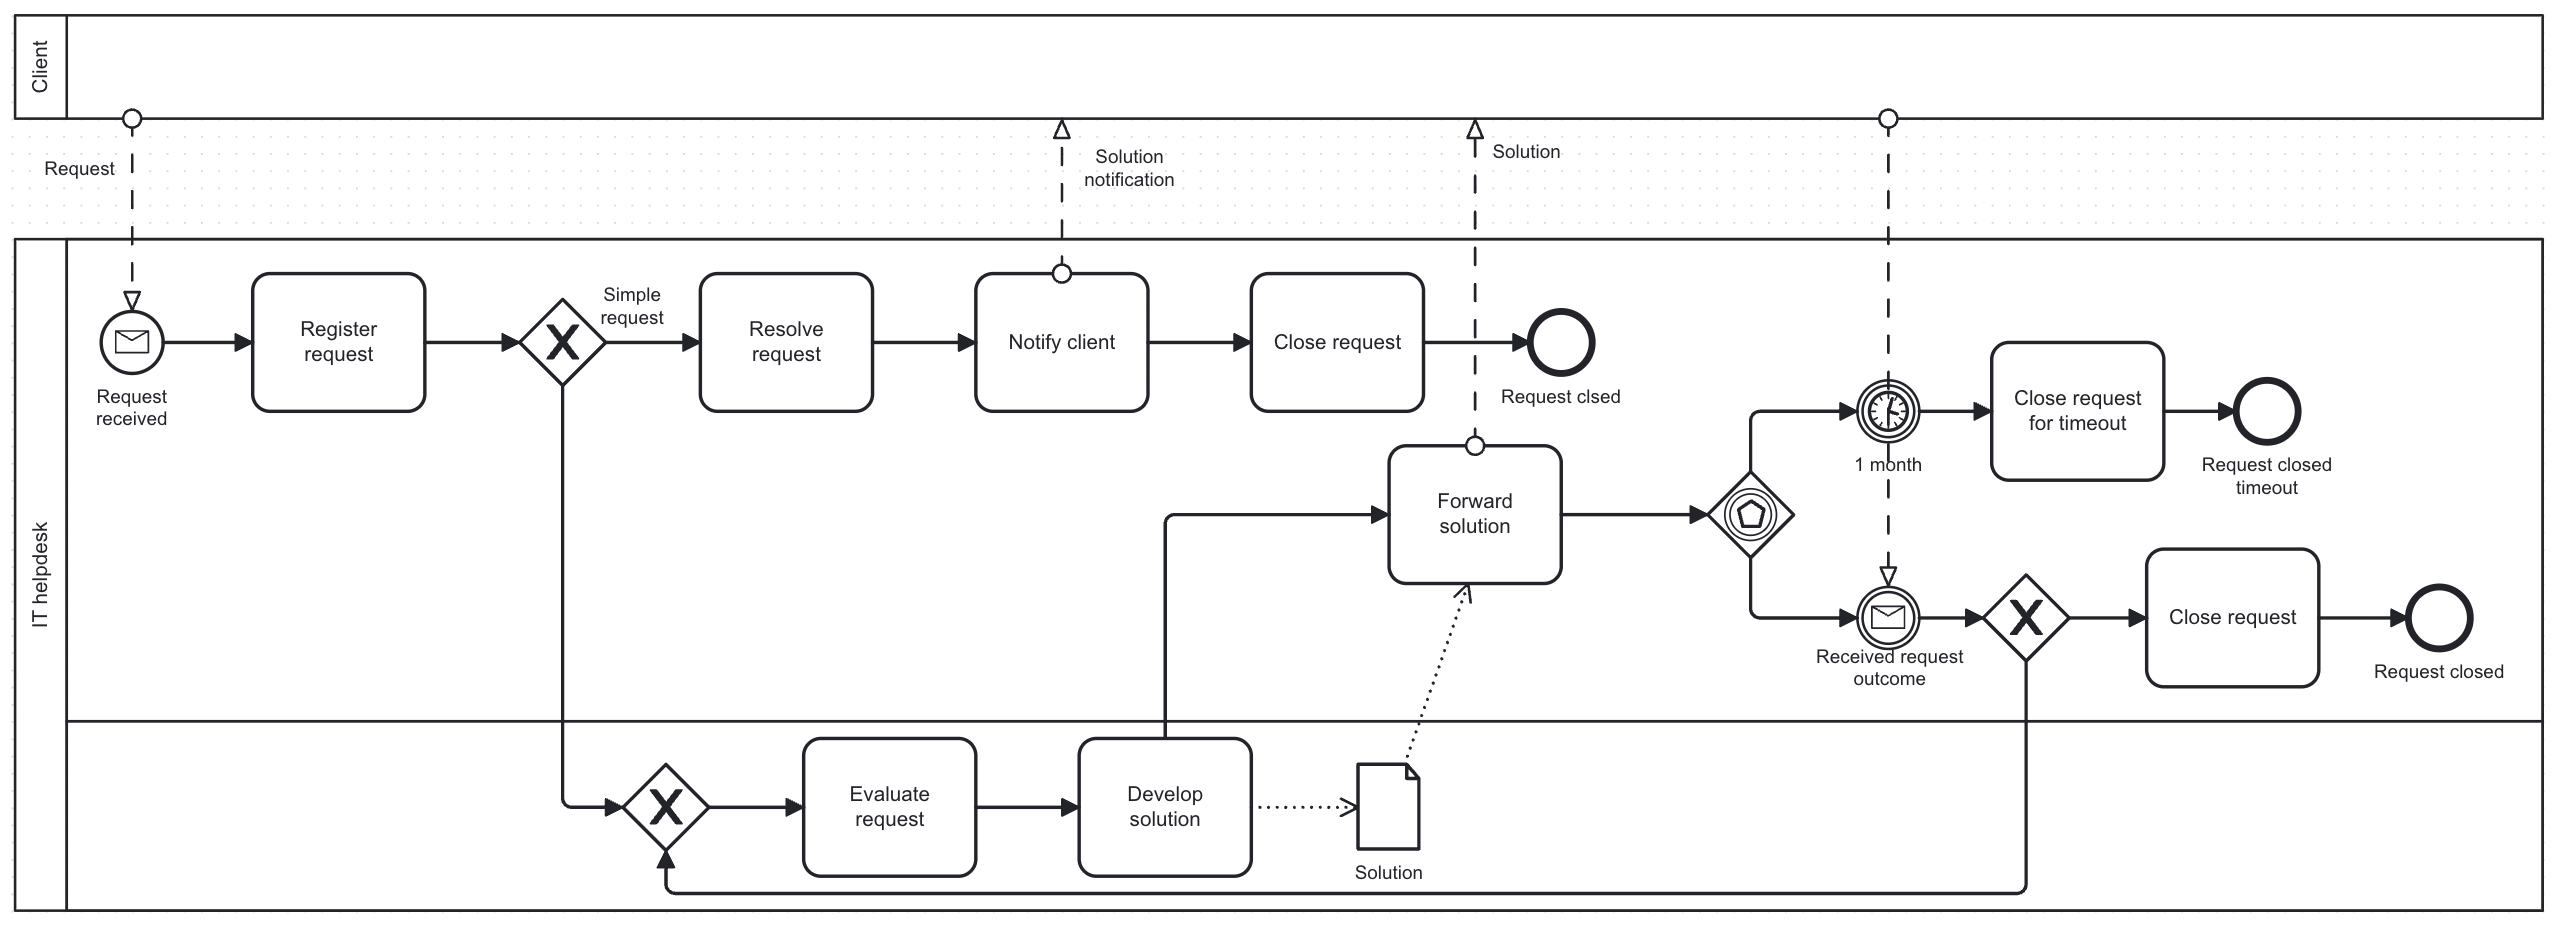
\includegraphics[width=\textwidth]{../images/exercises/bpmn/bpmn-7.png}
    \caption{Solution for Exercise 7}
\end{figure}
The important aspects of this solution are:
\begin{itemize}
    \item The process is modelled using 2 pools: the \textbf{Client} pool and the \textbf{IT Helpdesk} pool, 
    with two lanes: \textbf{Level-1 support} and \textbf{Level-2 support};
    \item The internal forwards of the request between Level-1 and Level-2 can be modelled using simple sequence flows;
    \item After forwarding the resolution to the client, the Level-1 support waits for an avent to happen:
    \begin{itemize}
        \item Either the client notifies that the request is fixed (intermediate message event);
        \item Or a timeout of one month occurs (intermediate timer event).
    \end{itemize}
    This is modelled using an event-based gateway, with the two intermediate events as outgoing branches;
    \item Before the evaluation of the request by Level-2 support, a XOR JOIN gateway is used, to allow repetition of the process.
\end{itemize}

\begin{exercise}{8}
Given the following process description, create a BPMN model that captures all the details:
\\\\After an expense report is received from an employee, the report is then reviewed for the approval. 
If the amount is lower than 1000 euros, it is automatically approved. 
If the amount is equal or higher than 1000 euros, then a manual check is required. 
In case the report is not ok, it is rejected and the employee has to be notified via email. 
In case it is fine, it is approved, the reimbursement is deposited to the employee’s bank account and the
documentation properly archived in parallel.
\end{exercise}
\paragraph{Solution:}
\begin{figure}[H]
    \centering
    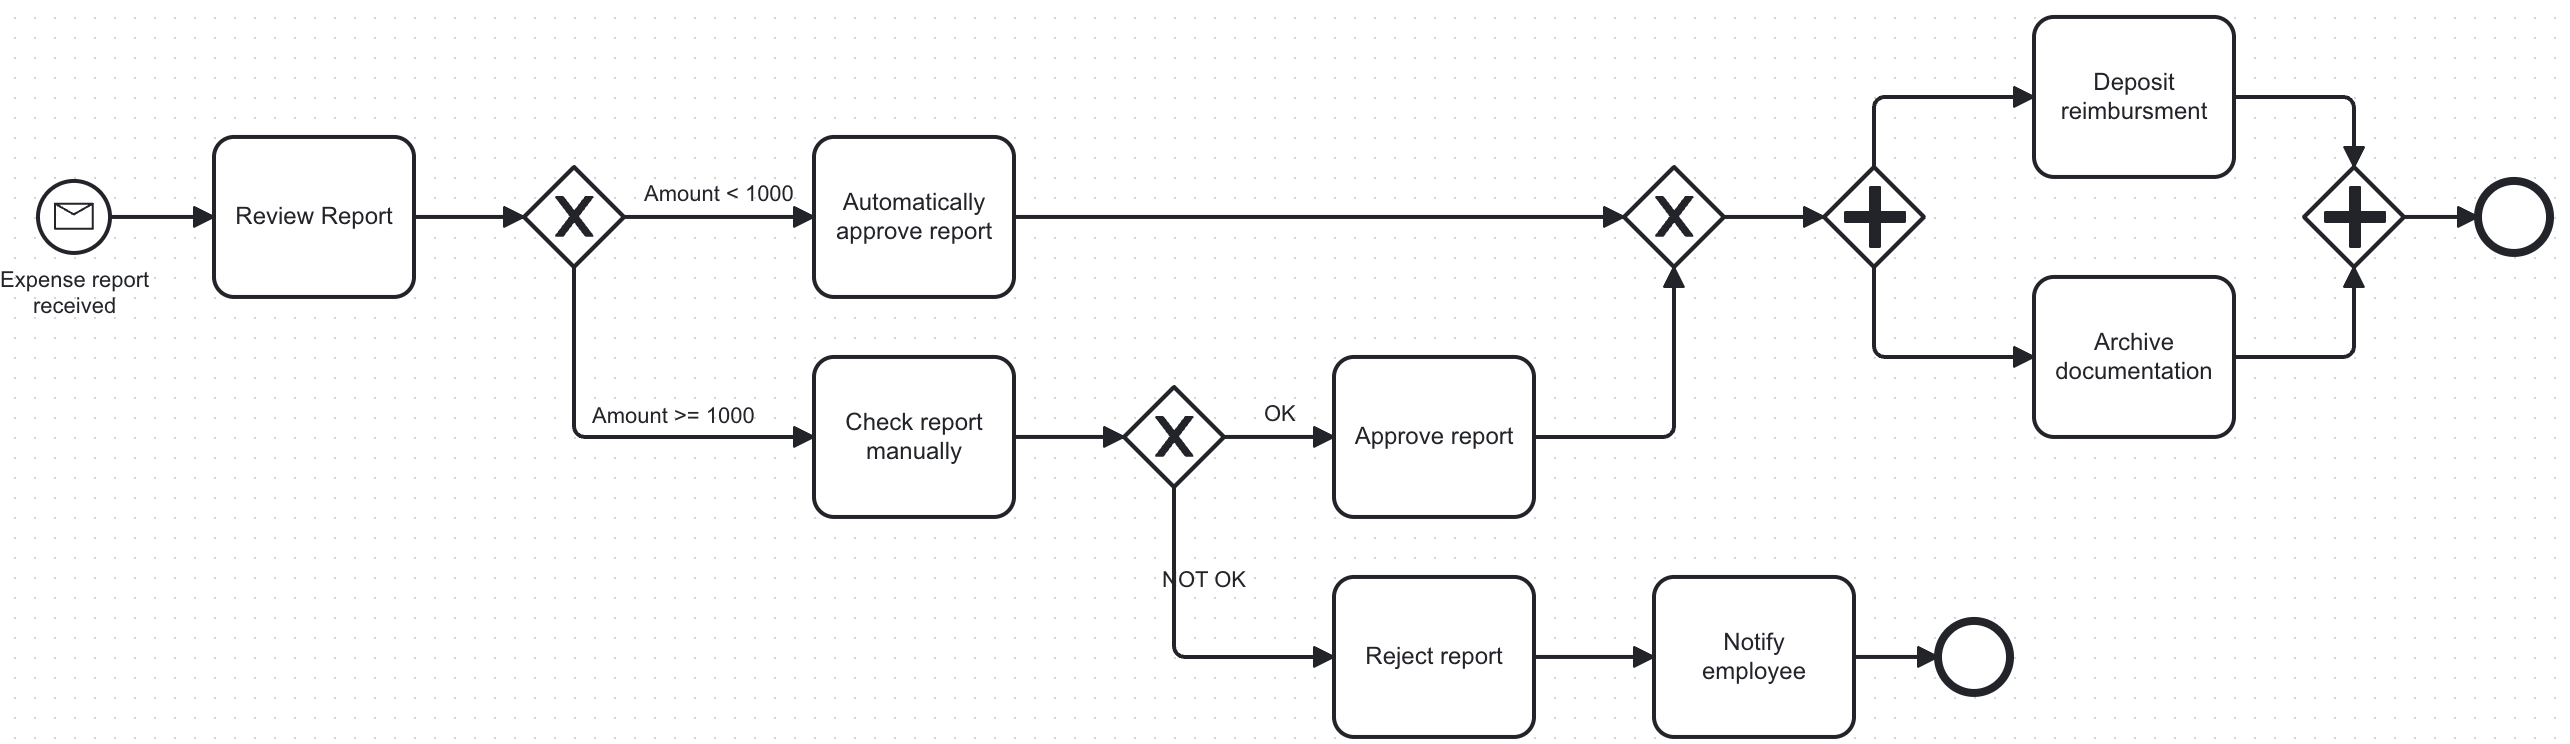
\includegraphics[width=\textwidth]{../images/exercises/bpmn/bpmn-8.png}
    \caption{Solution for Exercise 8}
\end{figure}

\begin{exercise}{9}
Given the following process description, create a BPMN model that captures all the details:
\\\\When a new credit request from the customer is received by the credit assessor, the risk level is checked. 
If the risk is above a threshold, an advanced risk assessment has to be carried out,
otherwise a simple risk assessment will suffice. 
Once the assessment has been completed, the customer is notified with the result of the assessment
and meantime, the disbursement is organized.
For simplicity we assume that the result of an assessment is always positive.
\end{exercise}
\paragraph{Solution:}
\begin{figure}[H]
    \centering
    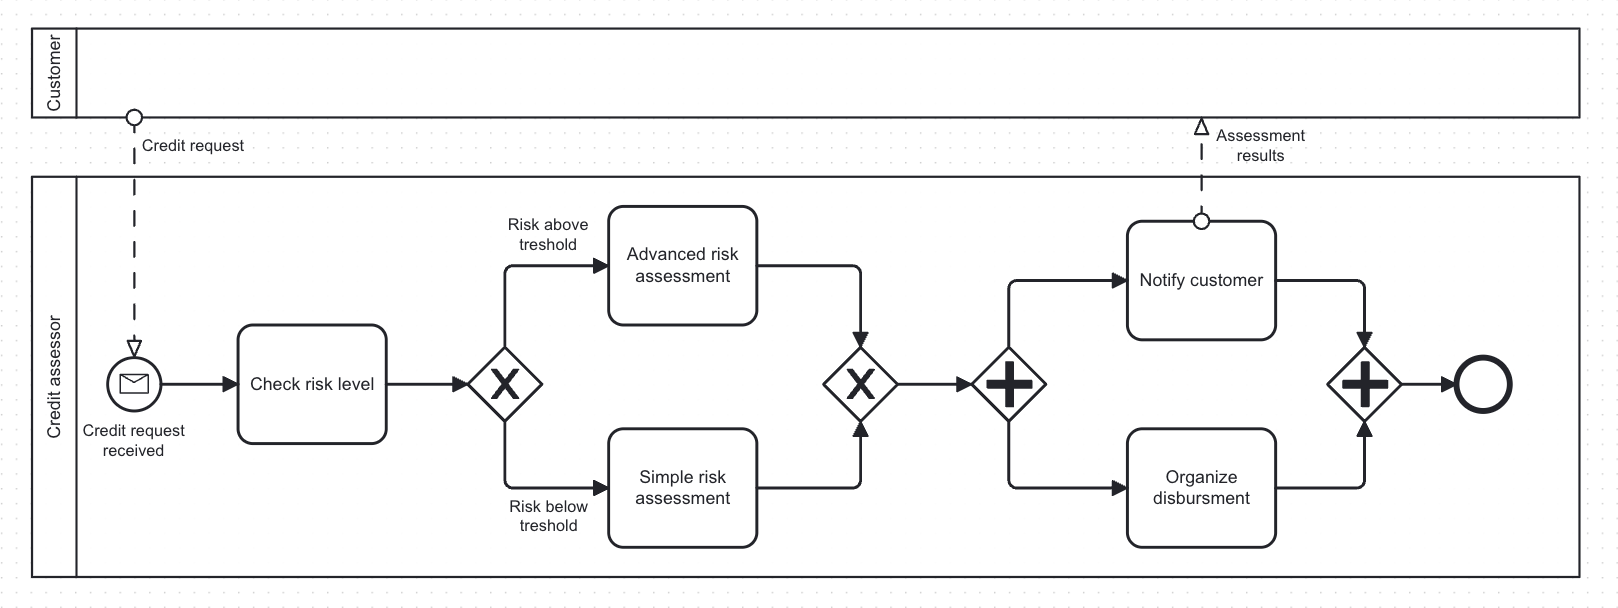
\includegraphics[width=\textwidth]{../images/exercises/bpmn/bpmn-9.png}
    \caption{Solution for Exercise 9}
\end{figure}
The important aspects of this solution are:
\begin{itemize}
    \item Since the text of the request mention both the customer and the credit assessor, we model them as two separate pools;
    \item A process instance starts with the receipt of a new credit request by the credit assessor (start message event). 
    We also need to model the message flow from the customer the start event;
    \item Since it's mentioned that the customer notification and the disbursement organization happen in parallel, we use an AND split gateway to model this;
    \item \textbf{OPTIONALLY}, we can add the data objects (credit request and assessment result) to the model to improve its understandability.
\end{itemize}

\begin{exercise}{10}
Given the following process description, create a BPMN model that captures all the details:
\\\\When a claim is received, it is registered. After registration, the
claim is classified leading to two possible outcomes: simple or
complex. If the claim is simple, the policy is checked. For complex
claims, both the policy and the damage are checked
independently.
A possible outcome of the policy check is that the insurance is
invalid. In this case, any processing is cancelled and a letter is sent
to the customer. In the case of a complex claim, this implies that
the damage checking is cancelled if it has not yet been
completed.
If, instead, the insurance is valid, an assessment is performed and,
in case of positive outcome the financial office is notified. Both in
case of positive and negative outcome, the customer is notified.
\end{exercise}
